\section{The \texorpdfstring{$\nim{2}$}{*2} Question}\label{sec:star2}

The $\nim{2}$ question of Section~\ref{sec:intro} asks whether a king-and-pawn position on a board with eight
ranks can have this value. We show that the only $\nim{2}$ in the census under the textbook test
comes from that test, that none exists with six pawns or fewer in the default setting, and that $\nim{2}$
appears with seven.

\subsection{The Textbook Candidate}

\begin{figure}[!t]
\centering
\begin{subfigure}{0.32\columnwidth}\centering
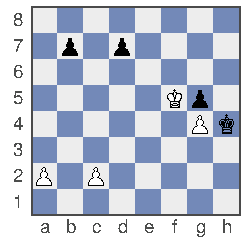
\includegraphics[width=\linewidth]{figures/star2_textbook.pdf}
\caption{Candidate}\label{fig:star2_textbook}
\end{subfigure}\hfill
\begin{subfigure}{0.32\columnwidth}\centering
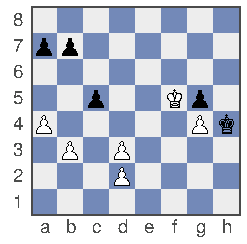
\includegraphics[width=\linewidth]{figures/star2_seven_a.pdf}
\caption{Position A}\label{fig:star2_seven_a}
\end{subfigure}\hfill
\begin{subfigure}{0.32\columnwidth}\centering
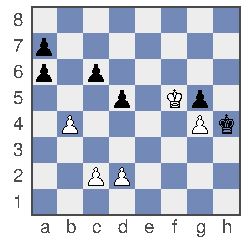
\includegraphics[width=\linewidth]{figures/star2_seven_b.pdf}
\caption{Position B}\label{fig:star2_seven_b}
\end{subfigure}
\caption{Positions of the $\nim{2}$ question beside T (Fig.~\ref{fig:trebuchet}; ordinary board). (a)~Candidate:
$\nim{2}$ under the textbook test, $\game{2\pm1}{-2\pm1}$ under the e.p.-aware test. (b)~Position A and
(c)~position B: $\nim{2}$ in the default setting (count rule, e.p.-aware test).}
\label{fig:star2}
\end{figure}

Fig.~\ref{fig:star2_textbook} shows the candidate \pos{W a2 c2 / B b7 d7} on files a--d. Under the count rule
with the textbook test, it is the only $\nim{k}$ with $k\ge2$ in the census of Section~\ref{sec:atlas}. If white
moves first, a2--a4 leaves $\star$ and c2--c4 leaves $0$; a2--a3 and c2--c3 are worse. The position is symmetric
(turn the board around and swap the colors), so black's d7--d5 leaves $\star$ and b7--b5 leaves $0$. Thus
$G=\game{0,\star}{0,\star}=\nim{2}$.

The weak point is black's plan b7--b5 and b5--b4. After b5--b4 the a-pawn is in the situation of
Fig.~\ref{fig:ep_test}: the textbook test scores a2--a4 as a passed pawn, $+\BIG$, but in chess black takes
b4$\times$a3 en passant. Under the e.p.-aware test, \pos{W a2 c2 / B b4 d7} is worth $-3$, a black win, so
b7--b5 is worth $-2\pm1$ and, by symmetry, c2--c4 is worth $2\pm1$. The other moves, among them a2--a4 and
d7--d5, which still lead to $\star$, are dominated or reversible. Hence
\[
G=\game{2\pm1}{-2\pm1},
\]
a hot game with mean $0$ and temperature $2$ \lab{C2}.

\subsection{No \texorpdfstring{$\nim{2}$}{*2} With Six Pawns or Fewer}

\begin{theorem}[Census; \lab{C2}]\label{thm:census}
In the census of Section~\ref{sec:atlas}, in the default setting, no position has value $\nim{k}$ with
$k\ge2$; the census has $6{,}724$ zeros and $4{,}042$ stars.
\end{theorem}

Our CGT engine and an independent C solver, which tests whether $G+\nim{k}$ is a second-player win, agree on
every record, and the independent whole-board solver finds no $\nim{k}$ with $2\le k\le 292$ among
$793{,}299$ labeled placements on widths 1--4 (every placement on each width, without reduction by symmetry or
translation). Every position in scope has birthday (Section~\ref{sec:notation}) at most $292$, so no
larger nimber can occur. Under the textbook test the census has $6{,}470$ zeros, $3{,}891$ stars and the
candidate; the e.p.-aware test removes that $\nim{2}$. In non-default settings a few other census
positions are $\nim{2}$; Section~\ref{sec:real-cand} tests one of them in real chess.

\subsection{\texorpdfstring{$\nim{2}$}{*2} With Seven Pawns}

\begin{theorem}[$\nim{2}$ with seven pawns; \lab{C2}]\label{thm:star2seven}
In the default setting, position~A, \pos{W a4 b3 d2 d3 / B a7 b7 c5}, and position~B,
\pos{W b4 c2 d2 / B a6 a7 c6 d5}, on files a--d of the ordinary board, have value $\nim{2}$, and both fit beside T, with the capture
histories c2$\times$d3 (A) and b7$\times$a6 (B). Neither is $\nim{2}$ with e.p.\ off or under the opponent rule.
\end{theorem}

In position A (Fig.~\ref{fig:star2_seven_a}), if white moves first, a4--a5 leaves $0$. The move d3--d4 attacks
c5; every black reply except c5$\times$d4 loses at once, and after c5$\times$d4 white continues b3--b4 to
$\star$, so the reversible move d3--d4 counts as a move to $\star$. White's third move, b3--b4, loses to
c5$\times$b4. If black moves first, a7--a5 leaves $0$ and b7--b6 leaves $\star$. Black's other moves are
reversible: after a7--a6 and b7--b5 white has replies worth $2$ and $3$, both at least $\nim{2}$; and c5--c4
lets d3$\times$c4 free white's d2 pawn for $+\BIG$. Thus
$G=\game{0,\star}{0,\star}=\nim{2}$.

In position B (Fig.~\ref{fig:star2_seven_b}), if white moves first, d2--d4 leaves $0$ and c2--c3 leaves
$\star$. The moves d2--d3 and c2--c4 are reversible, since black's replies reach $-2$ and $-3$, and b4--b5
loses to a6$\times$b5. If black moves first, d5--d4 leaves $0$, and a6--a5 attacks b4: every white reply except
b4$\times$a5 loses at once, and after b4$\times$a5 black continues c6--c5 to $\star$, so a6--a5 counts as a move
to $\star$. Black's third move, c6--c5, loses to b4$\times$c5. Thus $G=\nim{2}$ again.

\begin{table}[!t]
\centering
\caption{Values of the Three $\nim{2}$ Positions in the Model Settings}
\label{tab:star2_settings}
\footnotesize
\setlength{\tabcolsep}{4pt}
\begin{tabular}{@{}lccc@{}}
\toprule
Race rule, passed-pawn test & Candidate & A & B\\
\midrule
count, e.p.-aware & $\game{2\pm1}{-2\pm1}$ & $\nim{2}$ & $\nim{2}$\\
mover, e.p.-aware & $\game{2\pm1}{-2\pm1}$ & $\nim{2}$ & $\nim{2}$\\
count or mover, textbook & $\nim{2}$ & $\nim{2}$ & $\nim{2}$\\
count or mover, e.p.\ off & $\nim{2}$ & not $\nim{2}$ & not $\nim{2}$\\
opponent, any e.p.\ option & $0$ & not $\nim{2}$ & not $\nim{2}$\\
\bottomrule
\end{tabular}
\end{table}

In Table~\ref{tab:star2_settings} (e.p.\ on unless stated) every entry is \lab{C2}; for A and B, our CGT
engine, the census scanner that found them and the independent whole-board solver agree on each. The candidate
needs the textbook test but survives e.p.\ off; A and B need en passant but not the textbook test.

\subsection{Counts and Five Files}\label{sec:star2-five}

On ordinary boards of width at most four, in the default setting, two $\nim{2}$ positions have seven pawns and
four have eight. One exhaustive scan of $5{,}503{,}282$ root positions gives these counts, so their
completeness is \lab{C1}; our engine re-checked every position it reported \lab{C2}. With
Theorem~\ref{thm:census}, seven is the least number of pawns in a $\nim{2}$ on these boards \lab{C2}.

On five files a scan of all $14{,}680{,}983$ eight-pawn positions finds $21$ of value $\nim{2}$ in the default
setting \lab{C1}, each using all five files. As whole-board games all $21$ are $\nim{2}$: the whole-board solver
and our engine with splitting switched off agree \lab{C2}. As sums of components (Section~\ref{sec:sums-hss})
$15$ keep the value; the other six change only through the splitting. Three of the
$21$ come from the $14$ eight-pawn $\nim{2}$ rings on $\cyl{5}$ \lab{C1} by opening them onto files a--e:
\begin{itemize}
\item \pos{W a3 b3 c2 e2 / B a6 c5 d5 e3},
\item \pos{W a4 b3 c2 d2 / B a7 b6 c7 e4},
\item \pos{W a6 b4 c4 e3 / B a7 c7 d6 e6},
\end{itemize}
and these are $\nim{2}$ in both models. We call the first \emph{the five-file $\nim{2}$}. No $\nim{3}$ or higher nimber occurs in the default setting in any scope we searched
\lab{C1}.

By Theorem~\ref{thm:cut}, a pawn position on $\cyl{n}$ with an empty file is one on $\flatb{n-1}$, so these
scans also cover such positions on $\cyl{3}$ to $\cyl{5}$. A ring has no empty file. One scan of the rings on
$\cyl{5}$ to $\cyl{8}$ with at most eight pawns finds $\nim{2}$ in the default setting only in the $14$
eight-pawn rings on $\cyl{5}$ \lab{C1}. Narrower cylinders need fewer pawns. On $\cyl{3}$ the only ring
$\nim{2}$ with six pawns in the default setting is \pos{W a2 a3 b2 / B b7 c6 c7}, and on $\cyl{4}$ the first
are \pos{W a4 b2 c2 / B b6 c5 d6 d7} and its color-reversed twin, with seven; our engine confirms both values
\lab{C2}. No ring with fewer pawns is a $\nim{2}$ on either cylinder (the atlas up to five pawns, and a C scan
of every six- and seven-pawn split) \lab{C1}. On $\cyl{6}$ the first rings have nine pawns: a scan of every
nine-pawn ring finds six \lab{C1}, among them \pos{W a4 c4 d2 e2 / B b6 b7 d6 e5 f6}; both programs confirm
three, and the other three are their color-reversed twins \lab{C2}. So the first ring
$\nim{2}$ on $\cyl{n}$ has $n+3$ pawns for $n=3,\dots,6$. The $\cyl{3}$ ring needs en passant (with e.p.\ off its value is $0$), and it is a $\nim{2}$ with
one pawn fewer than any ordinary board of width at most four allows. Rings also carry $\nim{3}$, though not in
the default setting: with e.p.\ off, the eight-pawn ring \pos{W a5 b3 c2 d2 / B a7 b5 c6 d4} on $\cyl{4}$ is
$\nim{3}$ under the opponent rule, and the ten-pawn ring \pos{W a2 a3 b2 b3 c3 / B a6 a7 b6 b7 c6} on $\cyl{3}$
under the count rule \lab{C2}.

In the model, then, the $\nim{2}$ question has a positive answer on the ordinary $8\times8$ board: four files
and seven pawns beside T suffice, while Elkies' higher nimbers need larger boards~\cite{Elkies2002}. Whether real
chess agrees is the subject of Section~\ref{sec:real}.
